% Compile with: pdflatex lenses_diagram_simple.tex
% Block diagram of the 5 lenses with plain-English explanations
% Sized for 16:9 PowerPoint slide (13.33in x 7.5in).

\documentclass[11pt]{article}
\usepackage[paperwidth=13.33in, paperheight=7.5in, margin=8mm]{geometry}
\usepackage{tikz}
\usetikzlibrary{arrows.meta, positioning, calc, shadings, shapes}
\pagestyle{empty}

\definecolor{nlfFill}{RGB}{253, 230, 200}
\definecolor{nlfEdge}{RGB}{200, 130,  40}
\definecolor{cfaFill}{RGB}{220, 240, 215}
\definecolor{cfaEdge}{RGB}{ 80, 140,  70}
\definecolor{resFill}{RGB}{220, 232, 248}
\definecolor{resEdge}{RGB}{ 60, 110, 200}
\definecolor{lcaFill}{RGB}{248, 220, 232}
\definecolor{lcaEdge}{RGB}{195,  70, 120}
\definecolor{grayFill}{RGB}{238, 234, 226}
\definecolor{pcaFill}{RGB}{228, 222, 246}
\definecolor{pcaEdge}{RGB}{100,  80, 180}

\tikzset{
  lensbox/.style 2 args={
    draw=#2, fill=#1, rounded corners=4pt, line width=0.7pt,
    text width=185mm, align=left, inner sep=7pt,
    font=\sffamily,
  },
  endbox/.style={
    draw=black!40, fill=grayFill, rounded corners=4pt, line width=0.6pt,
    text width=26mm, align=center, inner sep=6pt,
    font=\sffamily\small,
  },
  pcabox/.style={
    draw=pcaEdge, fill=pcaFill!60, rounded corners=4pt, line width=0.6pt,
    text width=26mm, align=center, inner sep=6pt,
    font=\sffamily\small, text=pcaEdge!60!black,
  },
  flow/.style={
    -{Latex[length=2.4mm, width=2.2mm]}, semithick, draw=black!55,
  },
}

\newcommand{\lensline}[3]{%
  % #1 = title color, #2 = title text, #3 = body
  {\color{#1!70!black}\textbf{\large #2}}\\[2pt]
  \begin{minipage}{\linewidth}\sffamily\small
    #3
  \end{minipage}%
}

\newcommand{\citeline}[1]{%
  \\[1pt]{\footnotesize\itshape\color{black!55}#1}%
}

\begin{document}

\begin{center}
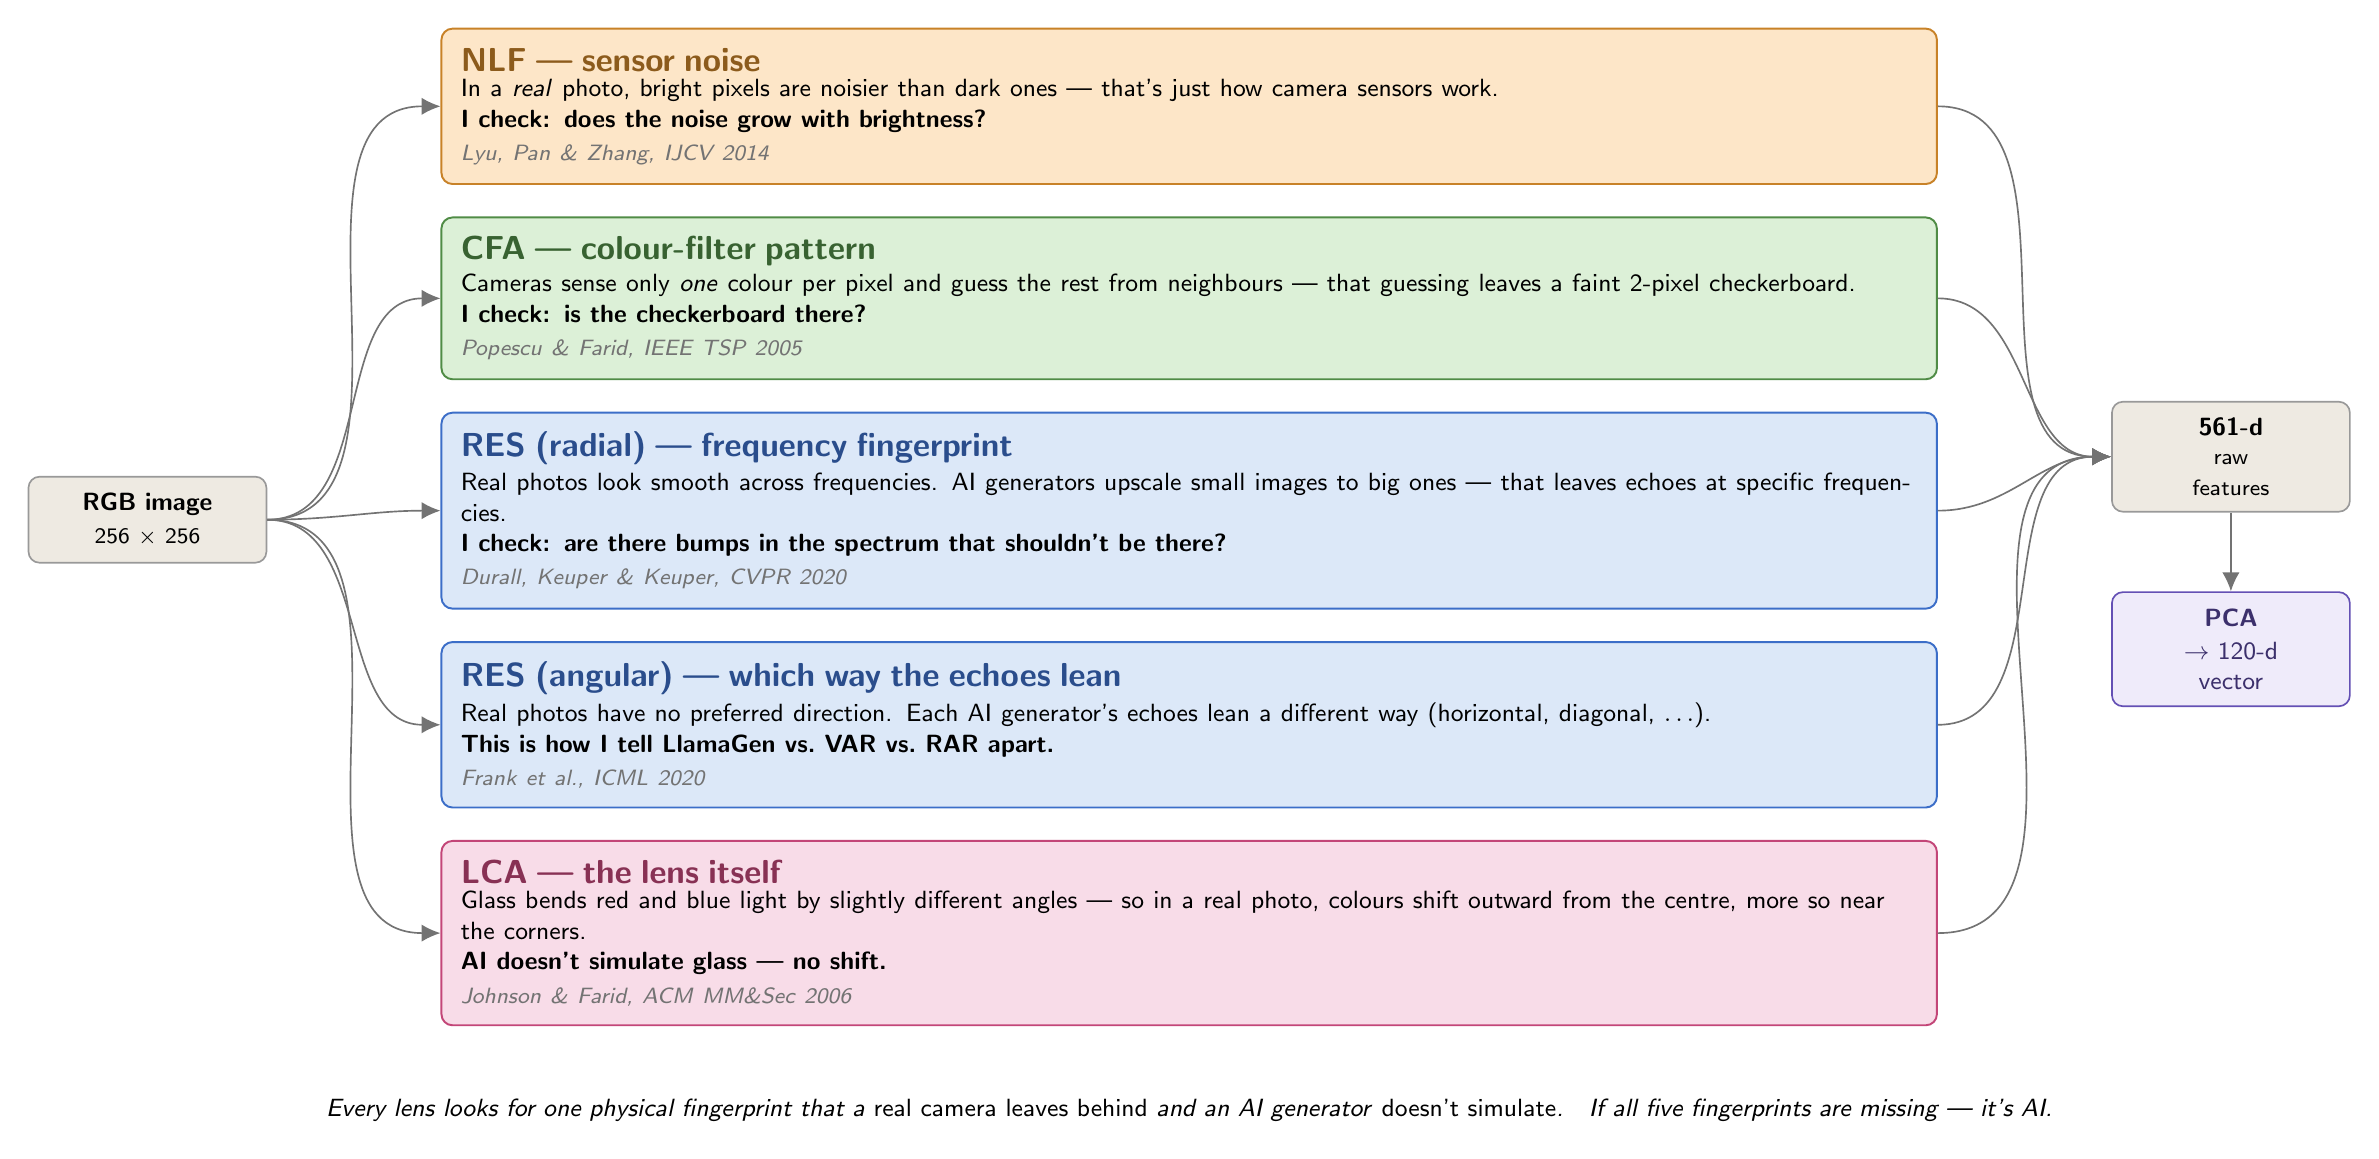
\begin{tikzpicture}[node distance=4mm]

% =========================================================================
% 5 lens boxes — stacked vertically, full slide width
% =========================================================================

\node[lensbox={nlfFill}{nlfEdge}] (nlf) {%
  \lensline{nlfEdge}{NLF --- sensor noise}{%
    In a \emph{real} photo, bright pixels are noisier than dark ones --- that's just how camera sensors work.\\
    \textbf{I check: does the noise grow with brightness?}%
    \citeline{Lyu, Pan \& Zhang, IJCV 2014}}};

\node[lensbox={cfaFill}{cfaEdge}, below=of nlf] (cfa) {%
  \lensline{cfaEdge}{CFA --- colour-filter pattern}{%
    Cameras sense only \emph{one} colour per pixel and guess the rest from neighbours --- that guessing leaves a faint 2-pixel checkerboard.\\
    \textbf{I check: is the checkerboard there?}%
    \citeline{Popescu \& Farid, IEEE TSP 2005}}};

\node[lensbox={resFill}{resEdge}, below=of cfa] (res1) {%
  \lensline{resEdge}{RES (radial) --- frequency fingerprint}{%
    Real photos look smooth across frequencies. AI generators upscale small images to big ones --- that leaves echoes at specific frequencies.\\
    \textbf{I check: are there bumps in the spectrum that shouldn't be there?}%
    \citeline{Durall, Keuper \& Keuper, CVPR 2020}}};

\node[lensbox={resFill}{resEdge}, below=of res1] (res2) {%
  \lensline{resEdge}{RES (angular) --- which way the echoes lean}{%
    Real photos have no preferred direction. Each AI generator's echoes lean a different way (horizontal, diagonal, $\ldots$).\\
    \textbf{This is how I tell LlamaGen vs.\ VAR vs.\ RAR apart.}%
    \citeline{Frank et al., ICML 2020}}};

\node[lensbox={lcaFill}{lcaEdge}, below=of res2] (lca) {%
  \lensline{lcaEdge}{LCA --- the lens itself}{%
    Glass bends red and blue light by slightly different angles --- so in a real photo, colours shift outward from the centre, more so near the corners.\\
    \textbf{AI doesn't simulate glass --- no shift.}%
    \citeline{Johnson \& Farid, ACM MM\&Sec 2006}}};

% =========================================================================
% RGB on the left, features + PCA on the right
% =========================================================================

\coordinate (boxes-mid) at ($(nlf.west)!0.5!(lca.west)$);

\node[endbox, left=22mm of boxes-mid] (rgb) {%
  \textbf{RGB image}\\[1pt]
  \footnotesize 256 $\times$ 256};

\coordinate (boxes-right) at ($(nlf.east)!0.5!(lca.east)$);

\node[endbox, right=22mm of boxes-right, yshift=8mm] (feat) {%
  \textbf{561-d}\\[1pt]
  \footnotesize raw\\features};

\node[pcabox, below=10mm of feat] (pca) {%
  \textbf{PCA}\\[1pt]
  $\rightarrow$ 120-d\\vector};

% =========================================================================
% arrows
% =========================================================================

\foreach \n in {nlf, cfa, res1, res2, lca}{
  \draw[flow] (rgb.east) to[out=0, in=180] (\n.west);
  \draw[flow] (\n.east)  to[out=0, in=180] (feat.west);
}
\draw[flow] (feat.south) -- (pca.north);

% =========================================================================
% tagline
% =========================================================================
\node[font=\sffamily\itshape\small, align=center, text width=290mm,
      below=8mm of lca.south, anchor=north]
   {Every lens looks for one physical fingerprint that a \emph{real camera leaves behind} and an AI generator \emph{doesn't simulate}.\quad
    If all five fingerprints are missing --- it's AI.};

\end{tikzpicture}
\end{center}

\end{document}
